% vim: set spell spelllang=en tw=100 et sw=4 sts=4 foldmethod=marker foldmarker={{{,}}} :

\documentclass{beamer}

\usepackage{tikz}
\usepackage{xcolor}
\usepackage{complexity}
\usepackage{hyperref}
\usepackage{microtype}
\usepackage{amsmath}                   % \operatorname
\usepackage{amsfonts}                  % \mathcal
\usepackage{amssymb}                   % \nexists
\usepackage{gnuplot-lua-tikz}          % graphs
\usepackage[vlined]{algorithm2e} % algorithms

\usetikzlibrary{shapes, arrows, shadows, calc, positioning, fit}
\usetikzlibrary{decorations.pathreplacing, decorations.pathmorphing, shapes.misc}
\usetikzlibrary{tikzmark}

\colorlet{screenverylightgrey}{black!2!white}
\colorlet{screengrey}{black!30!white}

\definecolor{uofguniversityblue}{rgb}{0, 0.219608, 0.396078}
\colorlet{uofguniversityblue40}{uofguniversityblue!40!white}

\definecolor{uofgheather}{rgb}{0.356863, 0.32549, 0.490196}
\definecolor{uofgaquamarine}{rgb}{0.603922, 0.72549, 0.678431}
\definecolor{uofgslate}{rgb}{0.309804, 0.34902, 0.380392}
\definecolor{uofgrose}{rgb}{0.823529, 0.470588, 0.709804}
\definecolor{uofgmocha}{rgb}{0.709804, 0.564706, 0.47451}

\definecolor{uofglawn}{rgb}{0.517647, 0.741176, 0}
\definecolor{uofgcobalt}{rgb}{0, 0.615686, 0.92549}
\definecolor{uofgturquoise}{rgb}{0, 0.709804, 0.819608}
\definecolor{uofgsunshine}{rgb}{1.0, 0.862745, 0.211765}
\definecolor{uofgpumpkin}{rgb}{1.0, 0.72549, 0.282353}
\definecolor{uofgthistle}{rgb}{0.584314, 0.070588, 0.447059}
\definecolor{uofgpillarbox}{rgb}{0.701961, 0.047059, 0}
\definecolor{uofglavendar}{rgb}{0.356863, 0.301961, 0.580392}

\colorlet{gp lt color 0}{uofguniversityblue}
\colorlet{gp lt color 1}{uofglavendar}
\colorlet{gp lt color 2}{uofglawn}
\colorlet{gp lt color 3}{uofgturquoise}
\colorlet{gp lt color 4}{uofgpumpkin}
\colorlet{gp lt color 5}{uofgsunshine}
\colorlet{gp lt color 6}{uofgcobalt}
\colorlet{gp lt color 7}{uofgpillarbox}

% {{{ theme things
\useoutertheme[footline=authortitle]{miniframes}
\useinnertheme{rectangles}

\setbeamerfont{block title}{size={}}
\setbeamercolor*{structure}{fg=uofguniversityblue}
\setbeamercolor*{palette primary}{use=structure,fg=black,bg=white}
\setbeamercolor*{palette secondary}{use=structure,fg=black,bg=uofguniversityblue40}
\setbeamercolor*{palette tertiary}{use=structure,fg=white,bg=uofguniversityblue}
\setbeamercolor*{palette quaternary}{fg=white,bg=black}

\setbeamercolor*{titlelike}{parent=palette primary}

\beamertemplatenavigationsymbolsempty

\tikzset{vertex/.style={draw, circle, inner sep=0pt, minimum size=0.5cm, font=\small\bfseries}}
\tikzset{notvertex/.style={vertex, color=white, text=black}}
\tikzset{plainvertex/.style={vertex}}
\tikzset{vertexc1/.style={vertex, fill=uofgthistle}}
\tikzset{vertexc2/.style={vertex, fill=uofgpumpkin}}
\tikzset{vertexc3/.style={vertex, fill=uofgpillarbox}}
\tikzset{vertexc4/.style={vertex, fill=uofgturquoise}}
\tikzset{edge/.style={color=screengrey}}
\tikzset{bedge/.style={ultra thick}}
\tikzset{edged/.style={color=screengrey, dashed}}
\tikzset{edgel3/.style={color=uofgturquoise, ultra thick}}

\setbeamertemplate{title page}
{
    \vbox{}
    \begin{center}
        {\usebeamerfont{title}\inserttitle\par}
        \vskip0.5cm\par
        \begin{beamercolorbox}[sep=8pt,center]{author}
            \usebeamerfont{author}\insertauthor
        \end{beamercolorbox}
        {\usebeamercolor[fg]{titlegraphic}\inserttitlegraphic\par}
    \end{center}
    \vfill

    \begin{tikzpicture}[remember picture, overlay]
        \node at (current page.north west) {\begin{tikzpicture}[remember picture, overlay]\fill
        [fill=uofguniversityblue, anchor=north west] (0, 0) rectangle (\paperwidth, -1.5cm);\end{tikzpicture}};
        \node [anchor=north west, shift={(0.2cm,-0.2cm)}] at (current page.north west) {\includegraphics*[keepaspectratio=true,scale=0.5]{UoG_keyline.eps}};
    \end{tikzpicture}
}

\setbeamertemplate{section page}
{
    \begin{centering}
        \begin{beamercolorbox}[sep=12pt,center]{part title}
            \usebeamerfont{section title}\insertsection\par
        \end{beamercolorbox}
    \end{centering}
}

\newcommand{\frameofframes}{/}
\newcommand{\setframeofframes}[1]{\renewcommand{\frameofframes}{#1}}

\makeatletter
\setbeamertemplate{footline}
{%
    \begin{beamercolorbox}[colsep=1.5pt]{upper separation line foot}
    \end{beamercolorbox}
    \begin{beamercolorbox}[ht=2.5ex,dp=1.125ex,%
        leftskip=.3cm,rightskip=.3cm plus1fil]{author in head/foot}%
        \leavevmode{\usebeamerfont{author in head/foot}\insertshortauthor}%
        \hfill%
        {\usebeamerfont{institute in head/foot}\usebeamercolor[fg]{institute in head/foot}\insertshortinstitute}%
    \end{beamercolorbox}%
    \begin{beamercolorbox}[ht=2.5ex,dp=1.125ex,%
        leftskip=.3cm,rightskip=.3cm plus1fil]{title in head/foot}%
        {\usebeamerfont{title in head/foot}\insertshorttitle}%
        \hfill%
        {\usebeamerfont{frame number}\usebeamercolor[fg]{frame number}\insertframenumber~\frameofframes~\inserttotalframenumber}
    \end{beamercolorbox}%
    \begin{beamercolorbox}[colsep=1.5pt]{lower separation line foot}
    \end{beamercolorbox}
}

% }}}

\title[The Subgraph Isomorphism Problem: Three New Ideas]{The Subgraph Isomorphism Problem: \\ Three New Ideas}
\author[Ciaran McCreesh]{\textcolor{uofguniversityblue}{Ciaran McCreesh} and Patrick Prosser}

\begin{document}

{
    \usebackgroundtemplate{\includegraphics*[keepaspectratio=true, height=\paperheight]{background.jpg}}
    \begin{frame}[plain,noframenumbering]
        \titlepage
    \end{frame}
}

\section{Subgraph Isomorphism}

\begin{frame}{The Subgraph Isomorphism Problem}

    \begin{itemize}
        \item Given a little \emph{pattern} graph and a large \emph{target} graph, find ``a copy
            of'' the pattern inside the target.

        \item We'll look at the \emph{non-induced} or \emph{monomorphism} variation: find an
            injective mapping that preserves adjacency, but not necessarily non-adjacency.
    \end{itemize}

    \vspace{2em}

    \centering
    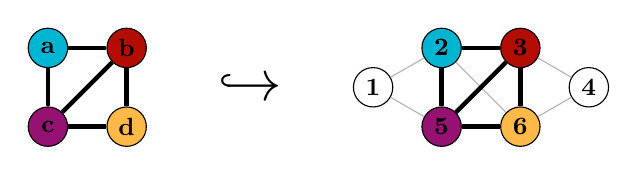
\begin{tikzpicture}
        \node [vertexc1] (Pc) at (0, 0) { c };
        \node [vertexc2] (Pd) at (1, 0) { d };
        \node [vertexc3] (Pb) at (1, 1) { b };
        \node [vertexc4] (Pa) at (0, 1) { a };

        \draw [bedge] (Pa) -- (Pb);
        \draw [bedge] (Pb) -- (Pc);
        \draw [bedge] (Pc) -- (Pd);
        \draw [bedge] (Pd) -- (Pb);
        \draw [bedge] (Pa) -- (Pc);

        \node [anchor=center, font=\huge] at (2.565, 0.5) { $\hookrightarrow$ };

        \node [vertex]   (T1) at (4.13, 0.5) { 1 };
        \node [vertexc1] (T5) at (5, 0) { 5 };
        \node [vertexc2] (T6) at (6, 0) { 6 };
        \node [vertexc3] (T3) at (6, 1) { 3 };
        \node [vertexc4] (T2) at (5, 1) { 2 };
        \node [vertex]   (T4) at (6.87, 0.5) { 4 };

        \draw [edge]  (T1) -- (T2);
        \draw [edge]  (T1) -- (T5);
        \draw [edge]  (T4) -- (T3);
        \draw [edge]  (T4) -- (T6);
        \draw [edge]  (T2) -- (T6);
        \draw [bedge] (T2) -- (T3);
        \draw [bedge] (T3) -- (T5);
        \draw [bedge] (T5) -- (T6);
        \draw [bedge] (T3) -- (T6);
        \draw [bedge] (T2) -- (T5);
    \end{tikzpicture}

\end{frame}

\begin{frame}{Existing Algorithms}
    \begin{itemize}
        \item VF2: widely used, and extremely fast on small, sparse, low degree graphs. But if
            it doesn't find a result within ten milliseconds, it is unlikely to find a result
            within a day.

        \item LAD and SND: very clever CP-like algorithms with deep reasoning. But for some
            larger target graphs, a single propagation takes over a second.

            \begin{itemize}
                \item We'll do much less reasoning, but can manage $>100,000$ propagations per
                    second.
            \end{itemize}
    \end{itemize}
\end{frame}

\begin{frame}{A CP-Like Model}

    \begin{itemize}
        \item One variable per vertex in the pattern graph. The domain is the vertex in the target
            graph that it gets mapped to.

        \item For each adjacent pair of vertices in the pattern graph, their values must be adjacent
            in the target graph.

        \item All variables have different values.

        \item We can filter initial domains using degree, neighbourhood degree sequence, loops,
            \ldots
    \end{itemize}

\end{frame}

\section{Supplemental Graphs}

\frame{\sectionpage}

\begin{frame}[b]{Distance-Based Filtering}

    \only<1> {
        \begin{itemize}
            \item If two vertices are distance $d$ apart in the pattern graph, they can only be mapped
                to a pair of vertices which are within distance $d$ (or less) in the target graph.
        \end{itemize}

        \vspace{2em}

        \centering
        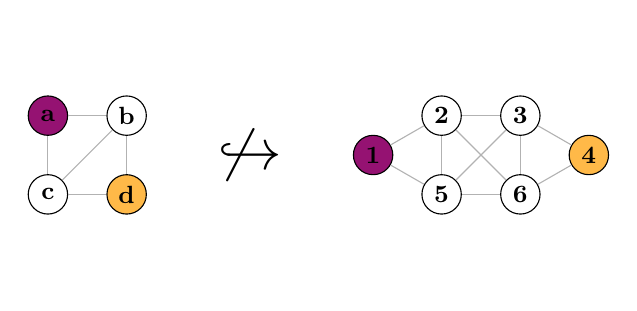
\begin{tikzpicture}
            \node [vertex] (Pc) at (0, 0) { c };
            \node [vertexc2] (Pd) at (1, 0) { d };
            \node [vertex] (Pb) at (1, 1) { b };
            \node [vertexc1] (Pa) at (0, 1) { a };

            \draw [edge] (Pa) -- (Pb);
            \draw [edge] (Pb) -- (Pc);
            \draw [edge] (Pc) -- (Pd);
            \draw [edge] (Pd) -- (Pb);
            \draw [edge] (Pa) -- (Pc);

            \node [anchor=center, font=\huge] at (2.565, 0.5) { $\not\hookrightarrow$ };

            \node [vertexc1] (T1) at (4.13, 0.5) { 1 };
            \node [vertex] (T5) at (5, 0) { 5 };
            \node [vertex] (T6) at (6, 0) { 6 };
            \node [vertex] (T3) at (6, 1) { 3 };
            \node [vertex] (T2) at (5, 1) { 2 };
            \node [vertexc2] (T4) at (6.87, 0.5) { 4 };

            \draw [edge] (T1) -- (T2);
            \draw [edge] (T1) -- (T5);
            \draw [edge] (T4) -- (T3);
            \draw [edge] (T4) -- (T6);
            \draw [edge] (T2) -- (T6);
            \draw [edge] (T2) -- (T3);
            \draw [edge] (T3) -- (T5);
            \draw [edge] (T5) -- (T6);
            \draw [edge] (T3) -- (T6);
            \draw [edge] (T2) -- (T5);

            \node at (5, 2) { ~ };
            \node at (5, -1) { ~ };
        \end{tikzpicture}

        \vspace{1em}
    }

    \only<2> {
        \begin{itemize}
            \item $G^d$ is the graph with the same vertex set as $G$, and an edge between $v$ and $w$ if the distance between $v$ and $w$ in $G$ is
                at most $d$.

            \item For any $d$, a subgraph isomorphism $i : P \hookrightarrow T$ is also a
                subgraph isomorphism $i^d : P^d \hookrightarrow T^d$.
        \end{itemize}

        \vspace{1em}

        \centering
        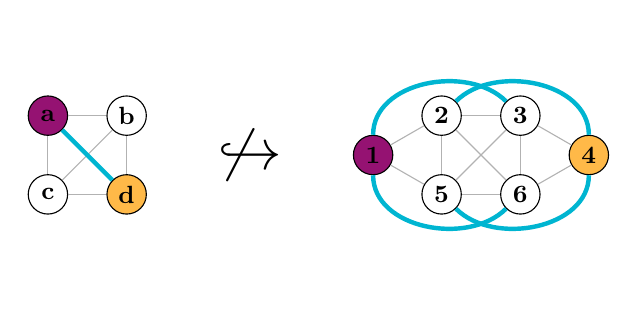
\begin{tikzpicture}
            \node [vertex] (Pc) at (0, 0) { c };
            \node [vertexc2] (Pd) at (1, 0) { d };
            \node [vertex] (Pb) at (1, 1) { b };
            \node [vertexc1] (Pa) at (0, 1) { a };

            \draw [edge] (Pa) -- (Pb);
            \draw [edge] (Pb) -- (Pc);
            \draw [edge] (Pc) -- (Pd);
            \draw [edge] (Pd) -- (Pb);
            \draw [edge] (Pa) -- (Pc);

            \draw [edgel3] (Pa) -- (Pd);

            \node [anchor=center, font=\huge] at (2.565, 0.5) { $\not\hookrightarrow$ };

            \node [vertexc1] (T1) at (4.13, 0.5) { 1 };
            \node [vertex] (T5) at (5, 0) { 5 };
            \node [vertex] (T6) at (6, 0) { 6 };
            \node [vertex] (T3) at (6, 1) { 3 };
            \node [vertex] (T2) at (5, 1) { 2 };
            \node [vertexc2] (T4) at (6.87, 0.5) { 4 };

            \draw [edge] (T1) -- (T2);
            \draw [edge] (T1) -- (T5);
            \draw [edge] (T4) -- (T3);
            \draw [edge] (T4) -- (T6);
            \draw [edge] (T2) -- (T6);
            \draw [edge] (T2) -- (T3);
            \draw [edge] (T3) -- (T5);
            \draw [edge] (T5) -- (T6);
            \draw [edge] (T3) -- (T6);
            \draw [edge] (T2) -- (T5);

            \draw [edgel3] (T1) to [in=135, out=90] (T3);
            \draw [edgel3] (T1) to [in=225, out=270] (T6);

            \draw [edgel3] (T4) to [in=45, out=90] (T2);
            \draw [edgel3] (T4) to [in=315, out=270] (T5);

            \node at (5, 2) { ~ };
            \node at (5, -1) { ~ };
        \end{tikzpicture}

        \vspace{1em}
    }
\end{frame}

\begin{frame}{Implied Constraints}
    \begin{itemize}
        \item We're now trying to find a mapping $i$ which is simultaneously a subgraph isomorphism
            \[
                \begin{array}{l@{\hskip 0.5cm}l@{\hskip 2mm}c@{\hskip 2mm}l@{\hskip 2mm}c@{\hskip 2mm}l}
                    &i &:& P &\hookrightarrow& T \\
                    \textnormal{and}& i^2 &:& P^2 &\hookrightarrow& T^2 \\
                    \textnormal{and}& i^3 &:& P^3 &\hookrightarrow& T^3
                \end{array}
            \] and so on.

        \item So we can filter on adjacency, degree, neighbourhood degree sequences, etc, in
            these graph pairs too.

        \item Open question: we can take the intersection, but is there a stronger operation
            which we can compute with reasonable complexity?
    \end{itemize}
\end{frame}

\begin{frame}{Path-Based Filtering}
    \begin{itemize}
        \item In practice, this only seems to be useful for $d \le 3$.

        \item Stronger: if two vertices in the pattern graph are connected by $k$ paths of
            length exactly $d$, then they can only be mapped to a pair of vertices which have at
            least $k$ paths of length exactly $d$ between them.

            \begin{itemize}
                \item We can also look at cycles: a vertex in a cycle of length $k$ must be mapped to a
                    vertex in a cycle of length $k$.
            \end{itemize}

        \item We can do this as using graph transformation too. Let $G^{\left[d, k\right]}$ be the
            (loopy) graph with the same vertex set as $G$, and an edge between $v$ and $w$ if there are at
            least $k$ paths or cycles of length exactly $d$ between $v$ and $w$ in $G$.

        \item This is \NP-hard to produce in general, but for $d \le 3$ and small $k$ we can
            calculate it quickly in practice.
    \end{itemize}
\end{frame}

\begin{frame}{Supplemental Graphs}
    \begin{itemize}
        \item We just build these graphs once, at the top of search.

            \begin{itemize}
                \item We could recreate them whenever a vertex disappears from every target domain,
                    but this is costly.

                \item We can cache these if we have a database of target graphs.
            \end{itemize}

        \item Other transformations are sometimes helpful. We can either pick a good, general set,
            or use domain knowledge.

        \item Different transformations are helpful for other variations of the problem.

            \begin{itemize}
                \item For the induced variant, we can also look at $\overline{G}$.
                \item And we can compose transformations.
            \end{itemize}
    \end{itemize}
\end{frame}

\begin{frame}{Is This Actually New?}
    \begin{itemize}
        \item SND uses distances (not paths) for filtering.

        \item Inference using $G^d$ is stolen from $k$-clique algorithms.
    \end{itemize}
\end{frame}

\section{Counting All-Different}

\frame{\sectionpage}

\begin{frame}{Injectivity / Enforcing All-Different}
    \begin{itemize}
        \item When assigning $D_v \gets w$, remove $w$ from every other domain. If a domain ends up
            being empty, fail and backtrack.

        \item This enforces the constraint, but does not provide much additional inference.
    \end{itemize}
\end{frame}

\begin{frame}{Hall Sets}
    \begin{itemize}
        \item If we have a subset of $n$ variables, whose domains include exactly $n$ values between
            them, then those values can \emph{only} be used by those variables.

        \item If we have a subset of $n$ variables, whose domains include less than $n$ values
            between them, then we cannot give every variable a different value.
    \end{itemize}
\end{frame}


\begin{frame}{R\'egin's Matching-Based All-Different Filtering}
    \begin{itemize}
        \item Build a bipartite graph, with variables on the left, values on
            the right, and edges for allowed assignments.

        \item Find a matching that covers every variable, or fail and backtrack if there isn't
            one.

        \item Remove every edge (variable-value assignment pair) which cannot occur in any
            maximum cardinality matching.
    \end{itemize}
\end{frame}

\begin{frame}{All-Different Filtering via Counting}
    \only<1> {
        \begin{itemize}
            \item Go through each variable, from smallest domain to largest, and take the union of
                the domains as we go along.

            \item If we reach a failed Hall set, fail.

            \item If we reach a Hall set, remove all these values from every remaining domain, reset
                the counters, and keep going.

            \item This is much faster, especially when domains are already bitsets, but may miss
                some deletions that matching would find.
        \end{itemize}
    }

    \only<2-11> {
        \centering
        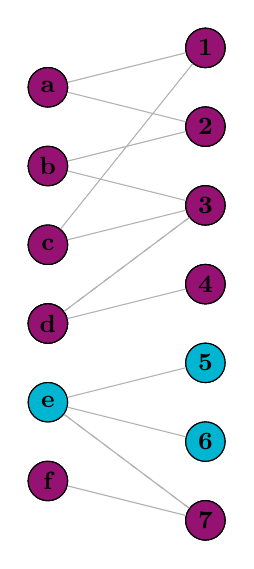
\begin{tikzpicture}

            \node <1-4>  [vertex]   (Va) at (0, 6) { a };
            \node <5-7>  [vertexc4] (Va) at (0, 6) { a };
            \node <8->   [vertexc1] (Va) at (0, 6) { a };

            \node <1-5>  [vertex]   (Vb) at (0, 5) { b };
            \node <6-7>  [vertexc4] (Vb) at (0, 5) { b };
            \node <8->   [vertexc1] (Vb) at (0, 5) { b };

            \node <1-6>  [vertex]   (Vc) at (0, 4) { c };
            \node <7>    [vertexc4] (Vc) at (0, 4) { c };
            \node <8->   [vertexc1] (Vc) at (0, 4) { c };

            \node <1-8>  [vertex]   (Vd) at (0, 3) { d };
            \node <9>    [vertexc4] (Vd) at (0, 3) { d };
            \node <10->  [vertexc1] (Vd) at (0, 3) { d };

            \node <10->  [vertexc1] (Vd) at (0, 3) { d };

            \node <1-10> [vertex]   (Ve) at (0, 2) { e };
            \node <11->  [vertexc4] (Ve) at (0, 2) { e };

            \node <2>    [vertex]   (Vf) at (0, 1) { f };
            \node <3>    [vertexc4] (Vf) at (0, 1) { f };
            \node <4->   [vertexc1] (Vf) at (0, 1) { f };

            \node <1-4>  [vertex]   (V1) at (2, 6.5) { 1 };
            \node <5-7>  [vertexc4] (V1) at (2, 6.5) { 1 };
            \node <8->   [vertexc1] (V1) at (2, 6.5) { 1 };

            \node <1-4>  [vertex]   (V2) at (2, 5.5) { 2 };
            \node <5-7>  [vertexc4] (V2) at (2, 5.5) { 2 };
            \node <8->   [vertexc1] (V2) at (2, 5.5) { 2 };

            \node <1-5>  [vertex]   (V3) at (2, 4.5) { 3 };
            \node <6-7>  [vertexc4] (V3) at (2, 4.5) { 3 };
            \node <8->   [vertexc1] (V3) at (2, 4.5) { 3 };

            \node <1-8>  [vertex]   (V4) at (2, 3.5) { 4 };
            \node <9>    [vertexc4] (V4) at (2, 3.5) { 4 };
            \node <10->  [vertexc1] (V4) at (2, 3.5) { 4 };

            \node <1-10> [vertex]   (V5) at (2, 2.5) { 5 };
            \node <11->  [vertexc4] (V5) at (2, 2.5) { 5 };

            \node <1-10> [vertex]   (V6) at (2, 1.5) { 6 };
            \node <11->  [vertexc4] (V6) at (2, 1.5) { 6 };

            \node <2>    [vertex]   (V7) at (2, 0.5) { 7 };
            \node <3>    [vertexc4] (V7) at (2, 0.5) { 7 };
            \node <4->   [vertexc1] (V7) at (2, 0.5) { 7 };

            \draw [edge] (Ve) -- (V5);
            \draw [edge] (Ve) -- (V6);
            \draw [edge] (Vd) -- (V4);
            \draw [edge] (Vc) -- (V3);
            \draw [edge] (Vc) -- (V1);
            \draw [edge] (Vb) -- (V2);
            \draw [edge] (Vb) -- (V3);
            \draw [edge] (Va) -- (V1);
            \draw [edge] (Va) -- (V2);
            \draw [edge] (Vf) -- (V7);

            \draw <2-7> [edge]  (Vd) -- (V3);
            \draw <8->  [edged] (Vd) -- (V3);

            \draw <2-3> [edge]  (Ve) -- (V7);
            \draw <4->  [edged] (Ve) -- (V7);

        \end{tikzpicture}
    }

    \only <12> {
        \begin{itemize}
            \item In this case we found both variable-value assignments which could never occur.

            \item Had we done tie-breaking in a different order, we could have missed one of these.
        \end{itemize}
    }
\end{frame}

\begin{frame}{Is This Actually New?}
    \begin{itemize}
        \item Claude-Guy Quimper and Toby Walsh used counting as preprocessing in the context of set
            variables, but they use it to determine whether it's worth trying a matching.

        \item Javier Larrosa and Gabriel Valiente counted neighbours for SIP.

        \item There are other propagators for bounds consistency.

        \item I can't find this variation in the literature, possibly because it doesn't enforce any
            particular kind of consistency.
    \end{itemize}
\end{frame}

\section{Backjumping}

\frame{\sectionpage}

\begin{frame}{Backtracking is Dumb}
    \begin{itemize}
        \item When we hit a failure, we could backtrack.
        \item Maybe the previous assignment didn't contribute to the failure, though.
    \end{itemize}
\end{frame}

\begin{frame}{Conflict-Directed Backjumping}
    \begin{itemize}
        \item Conflict-directed backjumping keeps a conflict set for each variable. We track
            which assignments removed a value from a variable. When we backtrack, if we did not
            cause the failure, we can keep going backwards.

        \item But copying conflict sets gives a performance hit inside a ``fast and dumb''
            algorithm.
    \end{itemize}
\end{frame}

\begin{frame}{Variable-Directed Backjumping}
    \begin{itemize}
        \item When we assign and fail, return which variables were involved in the failing
            constraint.

        \item When we cannot find any value to assign to a variable, return the union of the
            variables in failed sub-searches, plus ourself. (Intuition: we might be able to
            succeed, if either we had another value, or if another problematic variable had
            another value.)

        \item When a search subproblem fails, determine whether the assignment we just made
            removed any values from any of the failing variables. If not, jump back another step
            straight away.

            \begin{itemize}
                \item We don't need to track any additional information to do this, because we
                    have both the domains we were given, and the clone which has had propagation
                    applied to it.
            \end{itemize}
    \end{itemize}
\end{frame}

\begin{frame}{Backjumping plus All-Different}
    \begin{itemize}
        \item All-different(D) implies all-different(D') for any subset D' of D.

        \item If we can produce a small failed Hall set, we might be able to jump back further.

        \item We can just return the variables that we've seen so far.
            \begin{itemize}
                \item This sometimes helps a lot in practice.
                \item Maybe we could do more work to find an even better (not necessarily
                    smaller) set?
            \end{itemize}
    \end{itemize}
\end{frame}

\begin{frame}{Is This Actually New?}
    \begin{itemize}
        \item Current subgraph isomorphism algorithms just backtrack.

        \item Neil Moore implemented lazy explanation generation for CP, but in a different way.

        \item Guillaume Rochart, Narendra Jussien and François Laburthe worked out better
            explanations for all-different via flows, in the context of interactive CP.
    \end{itemize}
\end{frame}

\section{Preliminary Results}

\frame{\sectionpage}

\begin{frame}{Is This Any Good?}
    \begin{itemize}
        \item Fast and dumb isn't really fashionable for CP.

        \item Backjumping isn't fashionable anywhere\ldots

        \item We'll look at the 2063 benchmark instances used to evaluate LAD and SND.
            \begin{itemize}
                \item A mix of random, randomly structured, heavily structured, and real-world
                    graphs.
            \end{itemize}
    \end{itemize}
\end{frame}

\begin{frame}{Cumulative Performance}
    \input{gen-graph-cumulative}
\end{frame}

\begin{frame}{Per-Instance Comparison}
    \input{gen-graph-best-other}
\end{frame}

\begin{frame}{Is Each Feature Helpful?}
    \input{gen-graph-features}
\end{frame}

\begin{frame}{Is Backjumping Any Good?}
    \input{gen-graph-backjumping}
\end{frame}

\begin{frame}{How Much Worse is Counting All-Different?}
    \input{gen-graph-fad}
\end{frame}

\begin{frame}{Very Quick Attempt at Threaded Tree-Search}
    \only<1> {
        \begin{itemize}
            \item Half an hour's coding to check that the idea is sane.
            \item Distance 1 splitting to a queue, no extra load balancing yet.
            \item No parallelisation of supplemental graph construction yet.
            \item Speculative parallelism, so linear speedup should not be expected.
                \begin{itemize}
                    \item Not even for unsat instances, due to backjumping!
                \end{itemize}
            \item 16 threads.
        \end{itemize}
    }

    \only<2> {
        \input{gen-graph-speedup}
    }

    \only<3> {
        \input{gen-graph-parallel}
    }
\end{frame}

\begin{frame}{Proper Thread Parallelism?}
    \begin{itemize}
        \item Work order matters: parallel diversity is a good alternative to discrepancy search.

        \item Proper load balancing is necessary.

        \item Lack of parallel supplemental graph construction means we can't ignore
            Amdahl's law.

        \item Backjumping makes all this quite fiddly.
            \begin{itemize}
                \item It's easy to implement using Cilk, but we lose control of the work stealing
                    strategy.
                \item We could theoretically get an absolute slowdown due to backjumping. This is
                    preventable by not ``sharing backwards'', but might not be worth it.
            \end{itemize}
    \end{itemize}
\end{frame}

\begin{frame}{What's Next?}
    \begin{itemize}
        \item All the variants (labels, directed edges, induced, \ldots)

        \item Other supplemental graphs
            \begin{itemize}
                \item I can concoct additional transformations which can close half of the remaining
                    open instances, but they're rather specialised.
            \end{itemize}

        \item Portfolios and instance-specific algorithm configuration?
            \begin{itemize}
                \item Does this legitimise special transformations?
            \end{itemize}

        \item Symmetries and dominance?

        \item Better typesetting for $\overline{P} \not\hookrightarrow \overline{T}\,$?
    \end{itemize}
\end{frame}

\begin{frame}[b]
    \begin{center}
    \url{http://dcs.gla.ac.uk/~ciaran} \\
    \href{mailto:c.mccreesh.1@research.gla.ac.uk}{\nolinkurl{c.mccreesh.1@research.gla.ac.uk}}
\end{center}
\begin{tikzpicture}[remember picture, overlay]
    \node at (current page.north west) {\begin{tikzpicture}[remember picture, overlay]\fill
    [fill=uofguniversityblue, anchor=north west] (0, 0) rectangle (\paperwidth, -1.5cm);\end{tikzpicture}};
    \node [anchor=north west, shift={(0.2cm,-0.2cm)}] at (current page.north west) {\includegraphics*[keepaspectratio=true,scale=0.5]{UoG_keyline.eps}};
\end{tikzpicture}
\end{frame}

\end{document}

